% !TeX program = pdflatex
% One Engine, Three Counts -- Descartes, Sturm, Budan-Fourier through one sign-variation
% engine in Lean 4. Capstone/synthesis of the two prior papers (Sturm; Budan-Fourier),
% honest about classical unification (Akritas/BPR/Cauchy/Eisermann; Li-Paulson Isabelle).
% Reuses verified figures from figures/. Build: pdflatex (twice).

\documentclass[11pt]{article}
\usepackage[T1]{fontenc}
\usepackage{lmodern}
\usepackage{amsmath,amssymb,amsthm,booktabs,graphicx,hyperref}
\usepackage{xurl}
\usepackage[table]{xcolor}
\definecolor{ggteal}{HTML}{1B6F8C}
\definecolor{ggband}{HTML}{DCE7EB}
\definecolor{ggamber}{HTML}{E08A1E}
\definecolor{ggplum}{HTML}{7B4B94}
\usepackage[margin=1in]{geometry}
\usepackage{microtype}
\usepackage{float}
\usepackage[most]{tcolorbox}
\usepackage{tikz}
\usetikzlibrary{arrows.meta,positioning,fit,backgrounds,matrix}
\graphicspath{{figures/}}
\setlength{\emergencystretch}{2em}
\newtheorem{theorem}{Theorem}
\newtheorem{proposition}{Proposition}
\newtheorem{remark}{Remark}
\newcommand{\lean}[1]{\texttt{#1}}
\newcommand{\R}{\mathbb{R}}
\newcommand{\V}{\mathrm{V}}
\hypersetup{colorlinks=true,linkcolor=ggteal,citecolor=ggteal,urlcolor=ggteal}
\newtcbox{\keybox}{on line,boxrule=0.9pt,colframe=ggteal,colback=ggband!40,
  arc=3pt,left=8pt,right=8pt,top=5pt,bottom=5pt}
\newcommand{\keyeq}[1]{\begin{center}\keybox{$\displaystyle #1$}\end{center}}
\newtcolorbox{recipebox}[1]{colframe=ggamber,colback=ggamber!8,arc=3pt,boxrule=0.8pt,
  title=\textbf{#1},coltitle=white,colbacktitle=ggamber}

\title{\bf One Engine, Three Counts\\[4pt]
  \large\normalfont Descartes, Sturm and Budan--Fourier through one sign-variation engine in Lean~4}
\author{Carles Mar\'in\thanks{Formalized with the assistance of an AI system (Claude, Anthropic);
the mathematics is classical, every claim, scope statement and limitation is the author's
responsibility, and the Lean kernel---not the assistant---certifies the proofs. The boundary between
what is classical and what is contributed here is drawn explicitly in Section~\ref{sec:ours}.}\\[3pt]
  \normalsize Independent researcher\\
  \normalsize \texttt{karlesmarin@gmail.com}}
\date{June 2026}

\begin{document}
\maketitle

\begin{abstract}
Three classical theorems count the real roots of a polynomial in an interval by reading sign
variations of a sequence: \emph{Descartes'} rule uses the coefficients, \emph{Budan--Fourier} the
derivative tower $p,p',p'',\dots$, and \emph{Sturm} the signed-remainder chain. That they are facets
of one principle is classical (Akritas~\cite{akritas}; Basu--Pollack--Roy~\cite{bpr}), and the deepest
unifying invariant, the Cauchy index, is axiomatised through abstract \emph{Sturm chains} by
Eisermann~\cite{eisermann} and machine-checked, for the Cauchy-index route, in Isabelle/HOL by Li and
Paulson~\cite{liCauchy}. This paper does three things in Lean~4 over Mathlib, all \lean{sorry}-free.
(1)~It exhibits \emph{one engine}---a sign-variation count, its local constancy off critical points,
and a global telescoping over them---and runs all three theorems through it: the first Lean
formalizations of Sturm's theorem~\cite{sturmlean} and the Budan--Fourier theorem~\cite{budanlean},
and the bridge \lean{fourierVar p 0 = Polynomial.signVariations p} identifying the engine's $\V(0)$
with the coefficient sign count of Mathlib's own Descartes' rule, so the third count too is checked
against the library and not merely read off in prose. (2)~It states their common local-drop law,
$\V(c^-)=\V(c^+)+\mu_c+2e$, where $\mu_c$ is the order to which the counted polynomial vanishes at the
critical point $c$. (3)~It locates precisely where the three diverge: Eisermann's Sturm-chain axiom
forbids two consecutive members from vanishing together, and the derivative tower \emph{violates} this
at every multiple root, so the tower is \emph{not} a Sturm chain---its local law is the block
collapse/alternation (\lean{Rseq}/\lean{Lseq}), of which the antipodal single-drop of a genuine Sturm
chain is the non-degenerate special case. The unification is classical; the contribution is the shared
Lean engine, the two first-in-Lean formalizations it carries, the Descartes bridge to Mathlib's
coefficient count, and this exact axiomatic placement of the tower. Every headline theorem depends only on \lean{propext}, \lean{Classical.choice}, \lean{Quot.sound}.
\end{abstract}

\medskip
\noindent Three theorems, born a century and a half apart, count real roots by the same gesture:
reading the signs of a sequence. Descartes (1637) read them off the \emph{coefficients} and bounded the
positive roots. Budan (1807) and Fourier (1820s, published posthumously in 1831) read them off the
\emph{derivative tower}, extending the bound to any interval and counting with multiplicity; their
near-simultaneous discovery set off a priority dispute later disentangled by Akritas~\cite{akritas}.
Sturm (1829) closed the gap from bound to \emph{exact} count---but with a third sequence, the signed
Euclidean remainders, and only for distinct roots. That these are three faces of one principle emerged
only in the twentieth century, through Cauchy's index and its modern axiomatisation as abstract
\emph{Sturm chains} by Eisermann~\cite{eisermann}. \textbf{This paper makes that fusion concrete in
Lean: one sign-variation engine, one local-drop law, three instances run through it, and the exact point
where the derivative tower steps outside the Sturm-chain world.} The unification is classical; what is
new is the machine-checked engine and the axiomatic line it lets us draw between the three.

\medskip
\noindent\emph{What you will find here.} One engine (Section~\ref{sec:engine}); the local-drop law they
share (Section~\ref{sec:law}); the three instances read off it---Descartes, Sturm, Budan--Fourier
(Section~\ref{sec:three}); the dividing line, where the tower leaves the Sturm-chain world
(Section~\ref{sec:divide}); what is classical and what is contributed, without varnish
(Section~\ref{sec:ours}); and the questions worth carrying forward (Section~\ref{sec:open}). The two
companion papers~\cite{sturmlean,budanlean} carry the full proofs of the Sturm and Budan--Fourier
instances; here I assemble them into one picture and draw the line between them.

\begin{figure}[htbp]
\centering
\resizebox{\textwidth}{!}{%
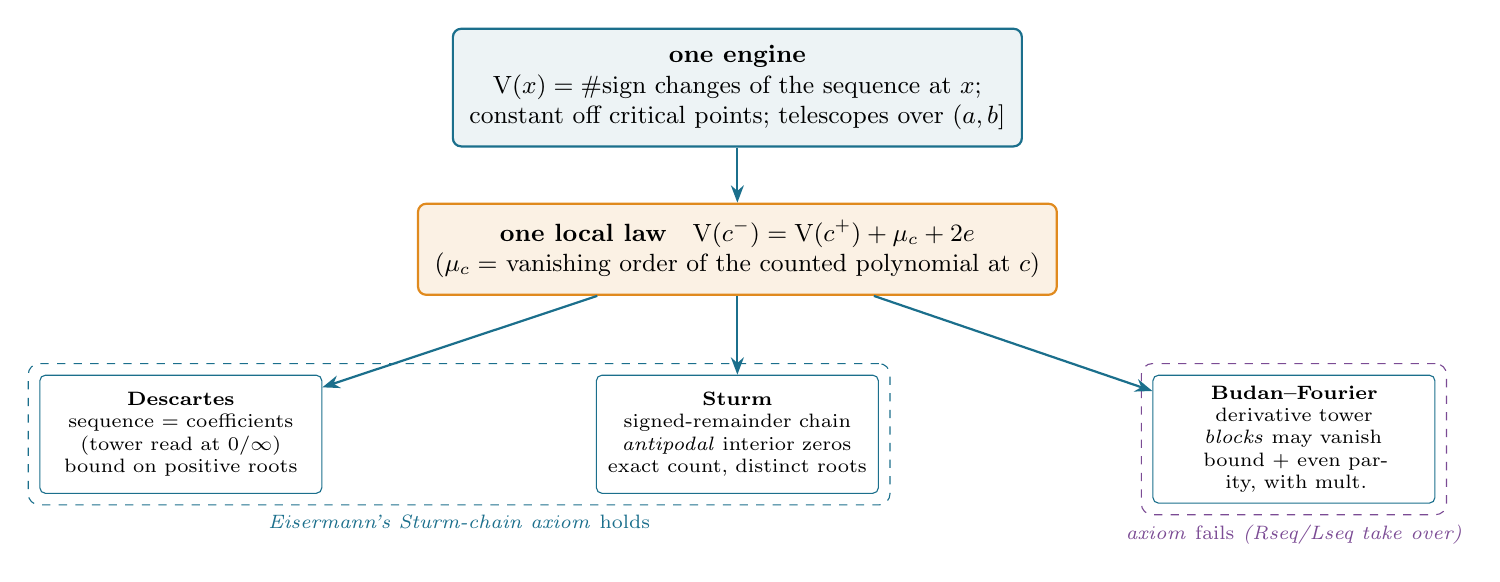
\begin{tikzpicture}[
  eng/.style={draw=ggteal,thick,rounded corners=3pt,fill=ggband!50,align=center,font=\small,
    inner sep=6pt},
  inst/.style={draw=ggteal,rounded corners=2pt,align=center,font=\scriptsize,inner sep=4pt,
    minimum height=15mm,text width=33mm,fill=white},
  law/.style={draw=ggamber,thick,rounded corners=3pt,fill=ggamber!12,align=center,font=\small,
    inner sep=6pt},
  arr/.style={-{Stealth[length=2.2mm]},thick,ggteal}]
  \node[eng] (engine) {\textbf{one engine}\\$\V(x)=\#$sign changes of the sequence at $x$;\\
    constant off critical points; telescopes over $(a,b]$};
  \node[law,below=7mm of engine] (law)
    {\textbf{one local law}\quad $\V(c^-)=\V(c^+)+\mu_c+2e$\\
     ($\mu_c=$ vanishing order of the counted polynomial at $c$)};
  \node[inst,below left=10mm and 12mm of law] (desc)
    {\textbf{Descartes}\\sequence $=$ coefficients\\(tower read at $0$/$\infty$)\\bound on positive roots};
  \node[inst,below=10mm of law] (sturm)
    {\textbf{Sturm}\\signed-remainder chain\\\emph{antipodal} interior zeros\\exact count, distinct roots};
  \node[inst,below right=10mm and 12mm of law] (bf)
    {\textbf{Budan--Fourier}\\derivative tower\\\emph{blocks} may vanish\\bound $+$ even parity, with mult.};
  \draw[arr] (engine) -- (law);
  \draw[arr] (law) -- (desc);
  \draw[arr] (law) -- (sturm);
  \draw[arr] (law) -- (bf);
  \begin{scope}[on background layer]
    \node[fit=(desc)(sturm),draw=ggteal,dashed,rounded corners=4pt,inner sep=4pt,
      label={[font=\scriptsize\itshape,text=ggteal]below:Eisermann's Sturm-chain axiom \emph{holds}}] {};
    \node[fit=(bf),draw=ggplum,dashed,rounded corners=4pt,inner sep=4pt,
      label={[font=\scriptsize\itshape,text=ggplum]below:axiom \emph{fails} (Rseq/Lseq take over)}] {};
  \end{scope}
\end{tikzpicture}}
\caption{The thesis in one picture. A single sign-variation engine and a single local-drop law carry
three classical root counts. Descartes' and Sturm's sequences obey Eisermann's Sturm-chain
axiom---no two members vanish together; the derivative tower of Budan--Fourier breaks it at every
multiple root and needs the block law \lean{Rseq}/\lean{Lseq}, of which the antipodal case is a
degeneration.}
\label{fig:thesis}
\end{figure}

\section{One engine}\label{sec:engine}

Fix a finite sequence of real polynomials $S=(S_0,\dots,S_n)$ and, for a point $x$ that is not a
common obstruction, let
\[
  \V_S(x)\ =\ \#\{\text{sign changes in } (\mathrm{sign}\,S_0(x),\dots,\mathrm{sign}\,S_n(x)),\ \text{zeros deleted}\}.
\]
In Lean this is one function, \lean{signChanges} on the list of evaluated signs (equivalently
\lean{signVarAt} on the polynomials), with one parity engine \lean{wallCount} underneath. Two facts hold
for \emph{any} such sequence of continuous functions and are proved once: \emph{(i)} on an interval
where no member vanishes, every sign is constant, so $\V_S$ is locally constant
(\lean{signVarAt\_eq\_of\_no\_root}, from the intermediate value theorem); \emph{(ii)} the parity of
$\V_S$ on a zero-free-ended block depends only on its first and last surviving signs
(\lean{wallCount\_even\_iff\_endpoints}). The \emph{critical points}---where some member vanishes---are
finite (the roots of $\prod_k S_k$, a nonzero polynomial), so $\V_S$ is a staircase: flat between
criticals, and the total descent over $(a,b]$ telescopes into a sum of per-critical drops. This
spine is shared verbatim by all three theorems; it was written once and used three times.

\section{One local law}\label{sec:law}

Everything then reduces to the drop across a single critical point $c$. Write $\V(c^-),\V(c^+)$ for the
locally-constant values just left and right of $c$, and let $\mu_c$ be the order to which the
\emph{counted} polynomial (the head $S_0=p$) vanishes at $c$. All three theorems are instances of one
statement.
\keyeq{\V(c^-)\ =\ \V(c^+)\ +\ \mu_c\ +\ 2e\qquad(\exists\,e\in\mathbb{N}).}
The right side carries no information beyond $c$ (the count just to the right equals the count at $c$
with zeros ignored); the left side adds the head's vanishing order $\mu_c$ and an \emph{even} surplus
$2e$ from the interior. Summing over the critical points in $(a,b]$ gives the interval statement: the
number of roots of $p$ there (with multiplicity $=\sum\mu_c$) is at most $\V(a)-\V(b)$, and differs from
it by the even $\sum 2e$. The whole divergence between the three theorems is in \emph{how the interior
behaves}---and that is exactly what the next two sections separate.

\section{Three instances}\label{sec:three}

We read all three off one worked polynomial where they can be compared, $p=x^3-x=x(x-1)(x+1)$, and then
name the feature each one isolates.

\emph{Sturm} (\cite{sturmlean}; Figure~\ref{fig:compare}). The signed-remainder chain
$x^3{-}x,\ 3x^2{-}1,\ \tfrac23 x,\ 1$ is built so that consecutive members are coprime: at a zero of an
interior member the two neighbours are \emph{antipodal} (strictly opposite), so deleting that member
leaves the count unchanged (the \lean{FlankReduce} relation). Only the head pair $(p,p')$ moves the
count, by one, at each root. The drop counts \emph{distinct} roots exactly: $\V(-2)-\V(2)=3$ on $(-2,2]$.
Here $\mu_c=1$ at every root and the surplus is $0$.

\emph{Budan--Fourier} (\cite{budanlean}; Figure~\ref{fig:compare}). The derivative tower
$p,p',p'',\dots$ replaces coprimality by a one-step relation---each member is the derivative of the
previous---so a vanishing member's sign just off $c$ is fixed by its derivative: it copies it on the
right (the block \emph{collapses}, no new change) and negates it on the left (the block
\emph{alternates}, one change per member). At a multiple root a whole block vanishes, the left
alternation contributes the multiplicity, and interior blocks contribute an even surplus---so the count
is a \emph{bound with multiplicity}, even-off from the truth. For $x^3-x$ (simple roots) it agrees with
Sturm; its distinctive face is the double root and the phantom even drop (Figure~\ref{fig:compare}).

\emph{Descartes} is the shadow at the ends of $(0,\infty)$: since $p^{(k)}(0)=k!\,a_k$, the tower's sign
sequence at $0$ \emph{is} the coefficient sequence, so $\V(0)$ is the coefficient sign-variation count;
and $\V(+\infty)=0$. The bound on positive roots is $\V(0)-\V(+\infty)=\V(0)$, even-off from the truth.
For $x^3-x$ the coefficients $1,0,-1,0$ give one sign change and one positive root, $x=1$. This last
instance is checked against the library, not just asserted: \lean{fourierVar p 0 =
Polynomial.signVariations p} (\lean{Descartes.lean}, \lean{sorry}-free), so the engine's $\V(0)$ is
\emph{definitionally} Mathlib's own coefficient sign-variation count---the function on which Mathlib's
Descartes' rule is stated. The bridge is the two facts above ($p^{(k)}(0)=k!\,a_k$, and
$\V(+\infty)=0$ left to prose) together with reversal-invariance of the sign count, the tower listing
the signs low-to-high and Mathlib's coefficient list high-to-low.

\begin{figure}[htbp]
\centering
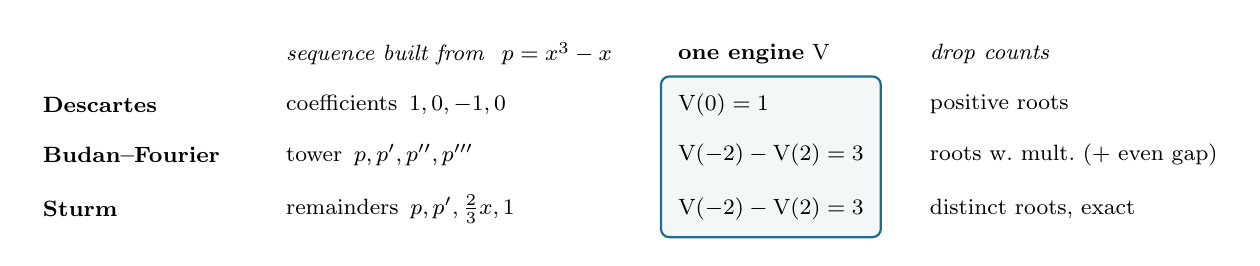
\begin{tikzpicture}[font=\footnotesize]
\matrix (m) [matrix of nodes, row sep=2.2mm, column sep=7mm, nodes={anchor=west, inner sep=2pt}]{
   & \textit{sequence built from } $p=x^3-x$ & \textbf{one engine} $\V$ & \textit{drop counts} \\
  \textbf{Descartes} & coefficients $\,1,0,-1,0$ & $\V(0)=1$ & positive roots \\
  \textbf{Budan--Fourier} & tower $\,p,p',p'',p'''$ & $\V(-2)-\V(2)=3$ & roots w.\ mult.\ ($+$ even gap) \\
  \textbf{Sturm} & remainders $\,p,p',\tfrac23 x,1$ & $\V(-2)-\V(2)=3$ & distinct roots, exact \\
};
\begin{scope}[on background layer]
  \node[draw=ggteal,thick,rounded corners=3pt,fill=ggband!35,fit=(m-2-3)(m-4-3),inner sep=4pt] {};
\end{scope}
\end{tikzpicture}
\caption{One polynomial, three sequences, one engine. Each classical count is the \emph{same}
sign-variation engine $\V$ applied to a different sequence built from $p=x^3-x$: Descartes'
coefficients, the Budan--Fourier derivative tower, Sturm's signed remainders. They read different
facets---positive roots, roots with multiplicity, distinct roots---but the count, its local constancy
off critical points, and its telescoping over $(a,b]$ are one and the same (boxed). The detailed
staircases live in the companion papers~\cite{sturmlean,budanlean}; this paper's subject is the boxed
column they share.}
\label{fig:compare}
\end{figure}

\section{The dividing line}\label{sec:divide}

What separates Sturm from Budan--Fourier is not a matter of taste; it is a precise axiom, and the
machine made it precise. Eisermann's abstract \emph{Sturm chain}~\cite{eisermann} is required to satisfy
one condition (his Def.~3.10): whenever an \emph{interior} member $S_k$ vanishes, its neighbours are
strictly opposite there,
\keyeq{S_k(c)=0\ \Longrightarrow\ S_{k-1}(c)\,S_{k+1}(c)<0\qquad(0<k<n),}
which in particular forbids two consecutive members from vanishing together. Sturm's chain satisfies it
(coprimality); Descartes' coefficient reading is degenerate but compatible.

\begin{proposition}[the derivative tower is not a Sturm chain]\label{prop:notsturm}
The derivative tower fails Eisermann's axiom at every multiple root. Concretely, for
$p_A=(x-1)^2(x+1)$ with tower $\big[p_A,\,p_A',\,p_A'',\,p_A'''\big]$, the interior member $p_A'$
vanishes at $x=1$, yet
\[
  p_A(1)\cdot p_A''(1)=0\cdot4=0\ \not<\ 0,
\]
because $p_A$ and $p_A'$ vanish there \emph{at once}. Hence the tower is not a Sturm chain in the sense
of~\cite{eisermann}, and the antipodal interior-deletion that proves Sturm's theorem cannot apply.
\end{proposition}

This is the whole point of the block law. Where a Sturm chain deletes one sandwiched interior member at
a time (\lean{FlankReduce}), the tower must resolve an entire vanishing block at once
(\lean{Rseq}/\lean{Lseq}: copy the derivative's sign on the right, negate it on the left). The two are
not rival techniques; the antipodal single-deletion is the \emph{non-degenerate special case} of the
block law, the case where every block has length one. Figure~\ref{fig:divide} sets the two local
geometries side by side.

\begin{figure}[htbp]
\centering
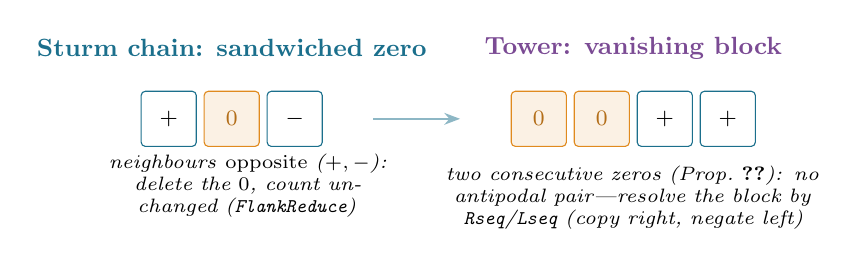
\begin{tikzpicture}[
  cell/.style={draw,rounded corners=1.5pt,minimum size=7mm,inner sep=1pt,font=\footnotesize},
  arr/.style={-{Stealth[length=2mm]},thick},
  lbl/.style={font=\scriptsize\itshape,align=center}]
  % Sturm side
  \node[font=\bfseries\small,text=ggteal] at (0.8,2.3) {Sturm chain: sandwiched zero};
  \node[cell,draw=ggteal] at (0,1.4) {$+$};
  \node[cell,draw=ggamber,fill=ggamber!12,text=ggamber!80!black] at (0.8,1.4) {$0$};
  \node[cell,draw=ggteal] at (1.6,1.4) {$-$};
  \node[lbl,text width=4.2cm] at (1.0,0.55)
    {neighbours \emph{opposite} ($+,-$): delete the $0$, count unchanged (\lean{FlankReduce})};
  % BF side
  \node[font=\bfseries\small,text=ggplum] at (5.9,2.3) {Tower: vanishing block};
  \node[cell,draw=ggamber,fill=ggamber!12,text=ggamber!80!black] at (4.7,1.4) {$0$};
  \node[cell,draw=ggamber,fill=ggamber!12,text=ggamber!80!black] at (5.5,1.4) {$0$};
  \node[cell,draw=ggteal] at (6.3,1.4) {$+$};
  \node[cell,draw=ggteal] at (7.1,1.4) {$+$};
  \node[lbl,text width=4.8cm] at (5.9,0.4)
    {two consecutive zeros (Prop.~\ref{prop:notsturm}): no antipodal pair---resolve the block by
     \lean{Rseq}/\lean{Lseq} (copy right, negate left)};
  \draw[arr,ggteal!50] (2.6,1.4) -- (3.7,1.4);
\end{tikzpicture}
\caption{Two local geometries. Left: a Sturm chain's interior zero sits between opposite signs and is
deleted without trace. Right: the tower's consecutive zeros have no such sandwich; the block is
resolved by collapse (right) and alternation (left). The first is the length-one special case of the
second.}
\label{fig:divide}
\end{figure}

\section{What is classical, and what is contributed}\label{sec:ours}

Without varnish. \emph{Classical, not ours}: that Descartes, Budan--Fourier and Sturm are facets of one
sign-variation principle (Akritas~\cite{akritas}; Basu--Pollack--Roy~\cite{bpr}); the Cauchy index as the
deep unifying invariant (Cauchy; Eisermann~\cite{eisermann}); and the abstract Sturm-chain axiomatisation
itself~\cite{eisermann}. \emph{Already machine-checked elsewhere}: the Cauchy-index route, in
Isabelle/HOL, by Li and Paulson~\cite{liCauchy}; and the Budan--Fourier theorem, in Isabelle/HOL, by
Li~\cite{liBF}. \emph{Contributed here}: the explicit \emph{shared} sign-variation engine in Lean~4 over
Mathlib; the first Lean formalizations of Sturm's theorem~\cite{sturmlean} and of Budan--Fourier~\cite{budanlean}
running through it; the bridge \lean{fourierVar p 0 = Polynomial.signVariations p}
(\lean{Descartes.lean}), which identifies the engine's $\V(0)$ with the coefficient sign count on which
Mathlib's own Descartes' rule is stated---so the third count is checked against the library, not merely
read off in prose; and Proposition~\ref{prop:notsturm}, the precise placement of the derivative tower
\emph{outside} the classical Sturm-chain axiom, with \lean{Rseq}/\lean{Lseq} identified as the local law
of that wider regime. Everything is over $\R$; the multiplicity step uses characteristic zero
essentially. No root is ever computed; no certificate is produced; no isolator is built.

\section{Questions worth carrying forward}\label{sec:open}

\begin{enumerate}\itemsep3pt
\item \emph{The weakest axiom.} Proposition~\ref{prop:notsturm} shows the tower escapes Eisermann's
condition. What is the \emph{weakest} hypothesis on an abstract sequence under which the local law
$\V(c^-)=\V(c^+)+\mu_c+2e$ still holds---one that has the antipodal Sturm-chain axiom and the derivative
tower as its two leading instances? A Lean structure carrying exactly that hypothesis would hold the
local lemma once instead of three times. The engine of Section~\ref{sec:engine} is already that
structure minus the local law; the law is what wants axiomatising.
\item \emph{Through the Cauchy index.} Li and Paulson formalised the Cauchy index in
Isabelle~\cite{liCauchy}; Mathlib has no such development. Does the engine here factor through a Lean
Cauchy index, recovering Sturm and Budan--Fourier as winding-number computations in the sense
of~\cite{eisermann}---and would the derivative tower then appear as a non-generic boundary case there too?
\item \emph{From bound to certificate.} The even surplus measures how far Budan--Fourier overshoots.
Can bisecting until it vanishes be turned into a verified, certificate-producing root isolator over
Mathlib, the multiplicity-aware analogue of the Vincent--Collins--Akritas methods~\cite{collinsakritas}?
\end{enumerate}

\noindent The pattern across all three is one reflection: the theorem is now a fixed point a kernel
defends, so the live direction is not to reprove it but to find the \emph{one} hypothesis of which the
three counts---and perhaps the Cauchy index above them---are instances, and to learn exactly how much of
it the derivative tower's blocks force us to weaken.

\section*{Reproducing}
\begin{verbatim}
git clone https://github.com/karlesmarin/godsil-gutman-lean
cd godsil-gutman-lean && lake exe cache get
lake env lean Sturm.lean          # the shared engine + Sturm instance
lake env lean BudanFourier.lean   # the Budan-Fourier instance (imports Sturm)
lake env lean Descartes.lean      # the Descartes bridge: V(0) = signVariations
\end{verbatim}
Lean \lean{v4.30.0-rc2}, Mathlib pin \lean{701fb6e9}. All headline theorems are \lean{sorry}-free and
\lean{\#print axioms} reports only \lean{propext}, \lean{Classical.choice}, \lean{Quot.sound}. The
worked signs of every figure are re-derived in exact arithmetic before the figure is drawn
(\lean{figures/}).

\begin{thebibliography}{99}\small
\bibitem{descartes} R.~Descartes, \emph{La G\'eom\'etrie} (1637).
\bibitem{budan} F.~D.~Budan de Boislaurent, \emph{Nouvelle m\'ethode pour la r\'esolution des
\'equations num\'eriques}, Paris (1807).
\bibitem{fourier} J.~Fourier, \emph{Analyse des \'equations d\'etermin\'ees}, Firmin Didot, Paris
(posthumous, 1831).
\bibitem{sturm} C.~Sturm, M\'emoire sur la r\'esolution des \'equations num\'eriques, \emph{M\'em.\
pr\'esent\'es par divers savants \`a l'Acad.\ Royale des Sci.} \textbf{6} (1835) 271--318.
\bibitem{akritas} A.~G.~Akritas, Reflections on a pair of theorems by Budan and Fourier, \emph{Math.\
Magazine} \textbf{55} (1982) 292--298.
\bibitem{collinsakritas} G.~E.~Collins, A.~G.~Akritas, Polynomial real root isolation using Descartes'
rule of signs, in \emph{Proc.\ SYMSAC~'76}, ACM, 1976, 272--275.
\bibitem{bpr} S.~Basu, R.~Pollack, M.-F.~Roy, \emph{Algorithms in Real Algebraic Geometry}, 2nd ed.,
Springer, 2006 (sign-variation theory, Ch.~2).
\bibitem{eisermann} M.~Eisermann, The fundamental theorem of algebra made effective: an elementary
real-algebraic proof via Sturm chains, \emph{Amer.\ Math.\ Monthly} \textbf{119} (2012), no.~9,
715--752; \texttt{arXiv:0808.0097}.
\bibitem{liBF} W.~Li, L.~C.~Paulson, Counting polynomial roots in Isabelle/HOL: a formal proof of the
Budan--Fourier theorem, in \emph{CPP~2019}, ACM, 2019, 52--64; \texttt{arXiv:1811.11093}.
\bibitem{liCauchy} W.~Li, L.~C.~Paulson, Evaluating winding numbers and counting complex roots through
Cauchy indices in Isabelle/HOL, \emph{J.~Automated Reasoning} \textbf{64} (2020), no.~2, 331--360;
\texttt{arXiv:1804.03922}.
\bibitem{mathlib} The mathlib Community, The Lean mathematical library, in \emph{CPP~2020}, ACM, 2020,
367--381.
\bibitem{lean4} L.~de Moura, S.~Ullrich, The Lean~4 theorem prover and programming language, in
\emph{CADE~28}, LNCS \textbf{12699}, Springer, 2021, 625--635.
\bibitem{sturmlean} C.~Mar\'in, \emph{The Staircase of Signs: Sturm's Root-Counting Theorem,
Machine-Checked in Lean~4}, Zenodo, 2026, \texttt{doi:10.5281/zenodo.20707348}.
\bibitem{budanlean} C.~Mar\'in, \emph{Counting with the Derivative Tower: The Budan--Fourier Theorem,
Machine-Checked in Lean~4}, Zenodo, 2026, \texttt{doi:10.5281/zenodo.20736143} (companion paper).
\end{thebibliography}

\end{document}
